\documentclass[12pt]{article}
\usepackage{geometry}
\usepackage{hyperref}
\geometry{a4paper, margin=1in}
\usepackage{graphicx}
\usepackage{tikz}
\usepackage{float}
\usepackage{caption}  % For caption formatting

\title{Software Requirements Specification (SRS)\\
\large \textbf{Real-Time Safety Monitoring System for Industrial Workplaces Using Deep Learning and Computer Vision}}
\author{
    Syed Ahad Ali \and Asad Ullah Chaudhry \and Muhammad Arsalan Hussain \and Muzzammil Kamran Sattar
}
\date{1st November 2024}
\begin{document}


\maketitle
\tableofcontents
\newpage





\section{Introduction}

\subsection*{Purpose}
This document aims to define the SRS requirement of the Dawlance Intenseye project. This system, designed for Dawlence’s sheet metal plant in Karachi, will continuously monitor workplace conditions via CCTV footage, detecting potential safety hazards in real time and issuing alerts to prevent workplace accidents. By analysing unsafe behaviours and maintaining compliance records, this system will enable Dawlance to identify and mitigate safety risks more proactively, ultimately fostering a safer work environment.

\subsection*{Scope}
The system will be deployed in the sheet metal plant of Dawlence in Karachi. It will process real-time video feeds from CCTV cameras, detecting safety hazards like improper personal protective equipment (PPE) usage, unsafe machinery operations, and obstacles in designated pathways. Notifications and alerts will be sent to workers and supervisors, with a web-based dashboard providing real-time monitoring and analytical insights. The scope of this document encompasses a detailed description of the final objectives of this project, the tasks which we, as students, will perform to achieve the objectives as well as the timeline in which all tasks will be completed and the team members responsible for each. We also mention the resources required for this project as well as a risk assessment of this project. We end by formalizing our functional requirements and non-functional requirements. 

During the project proposal presentation, we were given constructive feedback for improvement, which has been incorporated in this document and is mentioned below:

\begin{itemize}
    \item The Gantt chart now shows tasks that can be performed simultaneously, improving project efficiency.
    \item The Gantt chart now breaks down web development into multiple tasks, accurately reflecting the complexity of programming it.
\end{itemize}


\section{Project Plan}

\subsection*{Project Objectives}
The primary aim of this project is to develop and deploy a real-time monitoring system at Dawlence's sheet metal plant in Karachi. Our main objectives are:

\begin{itemize}
    \item \textbf{Safety Hazard Detection:} 
    \begin{itemize}
        \item The system will continuously analyse CCTV footage, identifying unsafe behaviours which include ensuring that:
        \begin{itemize}
            \item Workers wear mandatory PPE, including gloves and protective shoes.
            \item Workers avoid active machinery or other restricted areas by monitoring restricted zones.
            \item Walkways are clear of obstacles to avoid accidents.
            \item Machinery is not being operated unsafely or in an unapproved manner, which may result in harm.
            \item Safe distance is present between forklifts and workers.
        \end{itemize}
    \end{itemize}

    \item \textbf{Alert System for Quick Intervention:} 
    \begin{itemize}
        \item The system will feature an immediate alert/notification system that will inform on-site supervisors of any safety violations. Alerts will be delivered through multiple channels (dashboard, email, SMS).
    \end{itemize}
    
    \item \textbf{Data-Driven Safety Analysis:}
    \begin{itemize}
        \item Our project will include a dashboard displaying analytics of safety protocols and their breaches, which Dawlance can later use to identify trends and improve safety protocols and training over time.
        \item Gather footage from Dawlence's CCTV systems for the purpose of fine-tuning the model based on the hazard list provided by Dawlance.
        \item Supplement the dataset with publicly available industrial safety datasets to increase data variety, especially for scenarios underrepresented in the initial data collection.
    \end{itemize}
\end{itemize}

\subsection*{Project Tasks}
In order to complete the above objectives, this project can be divided into multiple tasks, some of which can be done in parallel and some in sequential order:

\begin{itemize}
    \item \textbf{Data Collection and Preparation}
    \begin{itemize}
        \item \textbf{Video Footage Collection:} Gather footage from Dawlence's CCTV systems for the purpose of fine-tuning the model based on the hazard list provided by Dawlance.
        \item \textbf{Public Data Integration:} Supplement the dataset with publicly available industrial safety datasets to increase data variety, especially for scenarios underrepresented in the initial data collection.
        \item \textbf{Data Annotation:} Label and annotate video data to categorize the video (with scenarios that require the fine-tuning).
    \end{itemize}

    \item \textbf{Model Development and Training}
    \begin{itemize}
        \item \textbf{Training and Fine-Tuning:} Use transfer learning and fine-tune YOLOv8 on annotated data, optimizing it to detect specific hazards accurately, such as identifying PPE compliance (e.g., gloves, helmets), restricted area breaches, and forklift operation safety.
    \end{itemize}

    \item \textbf{System Integration and Implementation}
    \begin{itemize}
        \item \textbf{Backend Development:} Develop a backend design that takes into account user roles, user access, and the data we wish to store. Integrate it with model outputs so the hazards that the model recognizes can be stored with data such as which camera it was captured on, the time, and the hazard type.
        \item \textbf{Frontend Development:} Develop a user-friendly, web-based dashboard using ReactJS for the front-end and NodeJS for the back-end. The dashboard will feature:
        \begin{itemize}
            \item \textbf{Real-Time Monitoring:} Safety compliance monitoring, visualized through live alerts and hazard notifications.
            \item \textbf{Safety Insights and Analytics:} Safety incident trends and analytics.
            \item \textbf{Embedded Camera Control:} Integrate camera functions (zoom, focus) to capture close-up footage of incidents as they happen, improving hazard identification.
            \item \textbf{Multi-Channel Notification System:} Build a robust notification system that supports alert channels such as in-dashboard notifications, emails, SMS, and alerts.
        \end{itemize}
    \end{itemize}

    \item \textbf{Post-Processing for Compliance Checks}
    \begin{itemize}
        \item \textbf{Hazard Contextualization:} Implement post-processing algorithms to assess detected hazards in context, differentiating between relevant and irrelevant situations (e.g., machinery that’s not actively in use doesn’t trigger alerts even if near workers).
    \end{itemize}

    \item \textbf{Testing and Optimization}
    \begin{itemize}
        \item \textbf{Factory Environment Testing:} Conduct pilot testing in Dawlence’s plant, adjusting the model for optimized performance in live industrial conditions.
        \item \textbf{Latency Optimization:} Ensure real-time system responsiveness by minimizing latency, so that alerts and notifications are sent with minimal delay.
    \end{itemize}

    \item \textbf{Documentation and Training}
    \begin{itemize}
        \item \textbf{Technical Documentation:} Provide comprehensive documentation detailing system setup, usage, maintenance, and troubleshooting, structured for both technical and non-technical users.
    \end{itemize}
\end{itemize}

\subsection*{Project Timeline}

\begin{figure}[H]
    \centering
    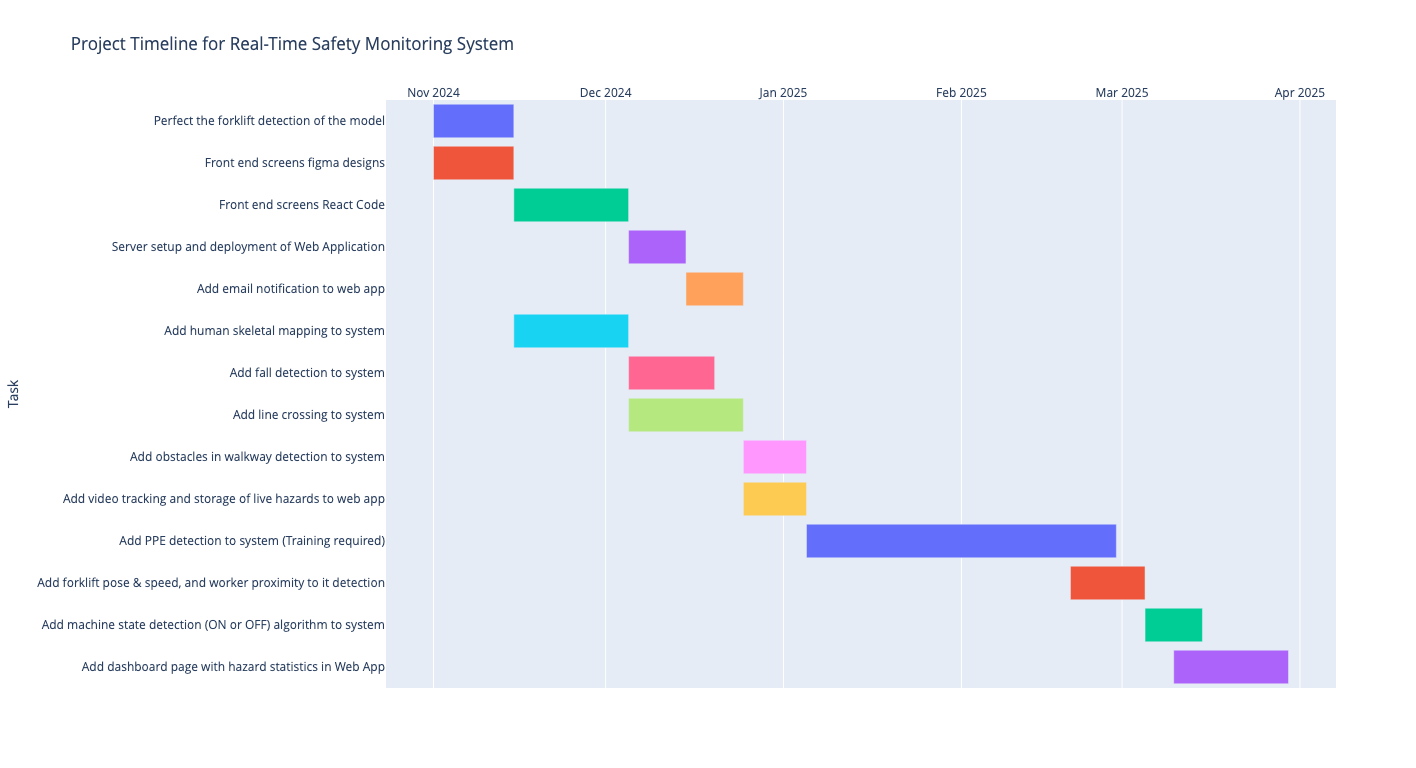
\includegraphics[width=1\textwidth]{gant.png} % Adjust width as needed
    \caption{Gantt Chart to Show Project Timeline}
    \label{fig:gant}
\end{figure}
\subsection*{Resources and Team Members}

\textbf{Technical Resources:}
\begin{itemize}
    \item \textbf{Hardware:} High-performance GPU for training, CCTV systems for video capture, and server infrastructure for real-time processing.
    \item \textbf{Software:} PyTorch for deep learning, OpenCV for computer vision, YOLOv8 for model training, MSSQL for data management, ReactJS for frontend development, NodeJS for backend.
    \item \textbf{Data:} A mix of Dawlence CCTV footage and supplementary datasets for diverse training data.
    \item \textbf{Models:} YOLOv8 and OpenCV.
\end{itemize}

\textbf{Team Members and Roles:}
\begin{itemize}
    \item \textbf{Muhammad Arsalan Hussain:} Specializes in deep learning with experience in dataset creation, AI model optimization, and leading development efforts, responsible for overseeing model training and fine-tuning.
    \item \textbf{Syed Ahad Ali:} Expertise in Software Engineering, trained in both large language models and camera control, focusing on full-stack development, model optimization, and camera integration.
    \item \textbf{Asad Ullah Chaudhry:} Data science background with experience in deep learning, responsible for data preparation, analysis, and insights generation while helping with model training and fine-tuning.
    \item \textbf{Muzzammil Kamran Sattar:} Skilled in software engineering, database design, and user interfaces, focusing on backend integration, database management, and front-end dashboard development.
\end{itemize}

\subsection*{Risks}

\begin{table}[h!]
\centering
    \begin{tabular}{|p{7cm}|p{7cm}|}
    \hline
    \textbf{Risks} & \textbf{Mitigation} \\
    \hline
    The limited availability of annotated safety data may impact model accuracy. & Use a mix of CCTV footage and public datasets, focusing on data diversity. \\
    \hline
    The project relies heavily on high-performance GPUs and additional CCTV setups. & Secure hardware resources through Dawlance and consider cloud-based GPU options if needed. \\
    \hline
    The model must balance accuracy with low latency for real-time monitoring. & Optimize YOLOv8 for speed, and refine post-processing filters to ensure reliable, responsive hazard detection. \\
    \hline
    Ensuring the system is adaptable to other environments may pose a challenge. & Emphasize modular design in both software and hardware to enable scalability across various industrial settings. \\
    \hline
    \end{tabular}
\end{table}



\section{Functional Requirements}

\subsection*{List of Functional Requirements}
\begin{enumerate}
    \item \textbf{Forklift Proximity Detection:} Relevant manager(s) should be notified via email and on web application if any worker is standing too close to a forklift.
    \item \textbf{Forklift Speed Estimation:} Relevant manager(s) should be notified via email and on web application if speed of any forklift goes above the company limit.
    \item \textbf{PPE Detection:} Relevant manager(s) should be notified via email and on web application if any worker is not wearing the appropriate safety equipment. Currently, the equipment is limited to gloves and shoes.
    \begin{enumerate}
        \item \textbf{Hazardous Area Entry Detection:} Relevant manager(s) should be notified via email and on web application if any worker is entering a hazardous area.
        \item Some areas are only considered hazardous if a certain machine in that area is operating. Thus, notifying should only take place if all the conditions are met including the operation of a machine.
    \end{enumerate}
    \item \textbf{Fall Detection:} Relevant manager(s) should be notified via email and on web application if any worker has fallen.
    \item \textbf{Climbing Detection:} Relevant manager(s) should be notified via email and on web application if any worker is climbing or has climbed.
    \item \textbf{Obstacle Detection:} Relevant manager(s) should be notified via email and on web application if there is presence of obstacles in walkway.
    \item \textbf{Statistics:} The dashboard of the web application should include data visualization of hazard detections made by the system:
    \begin{enumerate}
        \item Total detections made today and total detections made over the course of the month must be displayed.
        \item A pie chart must be displayed to illustrate the distribution of detected hazard types by percentage.
    \end{enumerate}
    \item \textbf{Video Feed:} The real-time annotated footage resulted from the hazard detection model(s) must be viewable for both cameras in the web application.
    \item \textbf{Notification System} The system will send real-time alerts through the dashboard to the supervisor about detected hazard and a textual description. The notification system shall support alerts via email, and web app notifications.
    \item \textbf{User Management:} The web application should include a user management system with the following features:
    \begin{itemize}
        \item \textbf{User Roles and Permissions:} Different levels of access for managers, supervisors, and regular users.
        \item \textbf{User Authentication:} Secure login process with multi-factor authentication.
    \end{itemize}
\end{enumerate}

\subsection*{Use Case Diagram}
\begin{figure}[H]
    \centering
    \includegraphics[width=1\textwidth]{usecase.jpg} % Adjust width as needed
    \caption{Use Case Diagram for Real-Time Safety Monitoring System}
    \label{fig:use_case_diagram}
\end{figure}


\section{System Overview}

\begin{itemize}
    \item \textbf{CCTV Cameras:} Positioned throughout the workplace, these cameras capture video feeds in real time for safety monitoring.

    \item \textbf{Hazard Detection AI Model(s) (YOLO):} These deep learning model(s) process the video feed to detect objects that are relevant to safety monitoring i.e. safety gloves, workers, forklift etc. This module can comprise of many different YOLO models that each perform their own specific object detection or it could comprise of just one or two consolidated models that detect many safety-relevant objects at once. The exact number of models cannot be estimated accurately but it will most likely be greater than one.

    \item \textbf{Backend Server:} Acts as the core of the system, coordinating between the CCTV feed, the hazard detection model, and the notification system. It manages data storage and API endpoints, ensuring data integrity and real-time communication with other system components.

    \item \textbf{Database:} A centralized storage solution that securely retains historical data, incident records, and safety analytics.

    \item \textbf{Post-Processing:} Provides additional contextual analysis to filter out irrelevant detections made by YOLO model(s) and accurately flag true hazard events. It ensures that alerts are sent only in relevant scenarios, such as when a machine is operating in a restricted zone.

    \item \textbf{Notification System:} A multi-channel alert system that can send real-time alerts through the web-based dashboard, email or even physical alarm devices to notify managers and supervisors of detected hazards. It provides both visual and textual details on each hazard, allowing quick and effective response.

    \item \textbf{Web-Based Dashboard:} A user-friendly interface for real-time monitoring, incident reporting, and data analysis. Built with Angular and Node.js, the dashboard includes safety analytics and historical data to help managers identify trends and patterns.
\end{itemize}

\begin{figure}[H]
\centering
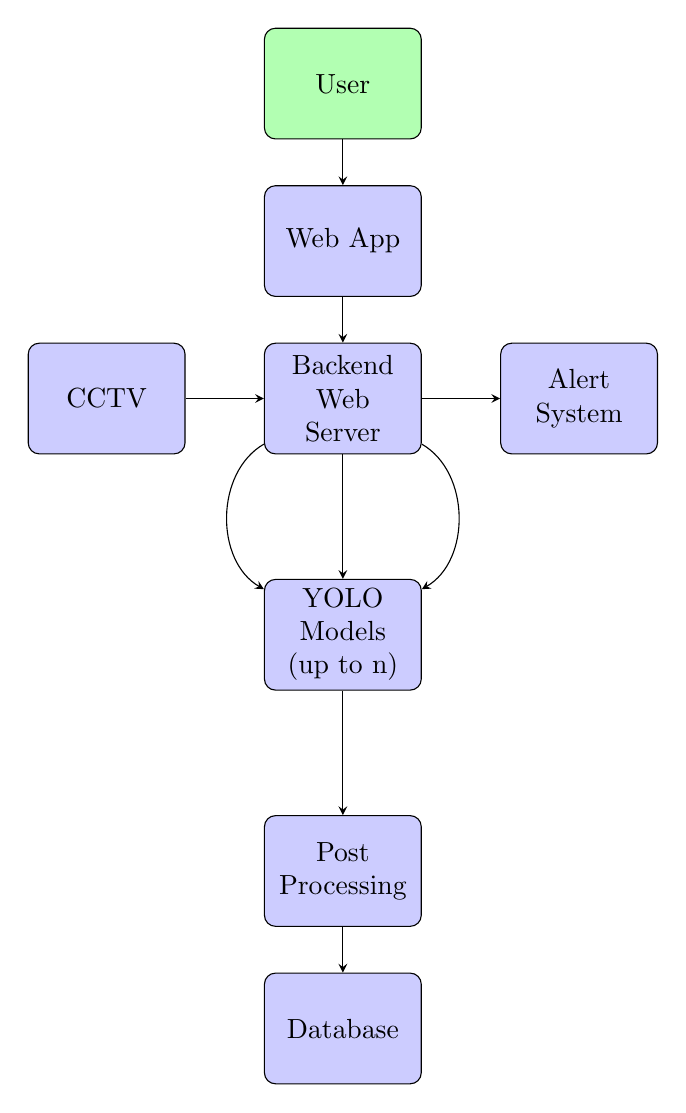
\begin{tikzpicture}
    % Define block styles
    \tikzstyle{block} = [rectangle, draw, fill=blue!20, 
        text width=5em, text centered, rounded corners, minimum height=4em]
    \tikzstyle{line} = [draw, -stealth] % Arrow with direction

    % Place nodes
    \node [block, fill=green!30] (user) {User};
    \node [block, below of=user, node distance=2cm] (webapp) {Web App};
    \node [block, below of=webapp, node distance=2cm] (backend) {Backend Web Server};
    \node [block, left of=backend, node distance=3cm] (cctv) {CCTV};
    \node [block, right of=backend, node distance=3cm] (alert) {Alert System};    
    \node [block, below  of=backend, node distance=3cm] (yolo) {YOLO Models (up to n)};
    \node [block, below of=yolo, node distance=3cm] (postproc) {Post Processing};
    \node [block, below of=postproc, node distance=2cm] (database) {Database};

    % Draw arrows
    \path [line] (user) -- (webapp);
    \path [line] (webapp) -- (backend);
    \path [line] (cctv) -- node[above] {} (backend);
    \path [line] (backend) -- node[above] {} (alert);
    \path [line] (backend) -- node[right] {} (yolo);
    \path [line] (yolo) -- node[right] {} (postproc);
    \path [line] (postproc) -- (database);
    % \path [line] (postproc) -- node[right] {} (alert);
    
    % Additional arrows for YOLO to WebApp
    \path [line] (backend) to[out=210,in=150] (yolo); % Arrow from WebApp to YOLO
    \path [line] (backend) to[out=-30,in=30] (yolo);  % Arrow from WebApp to YOLO
    
\end{tikzpicture}
\caption{Directed System Block Diagram}
\label{fig:directed_block_diagram}
\end{figure}




\section{Non-Functional Requirements}

\subsection*{Performance}
\begin{itemize}
    \item The system should process video and detect safety hazards in real-time with a maximum latency of 5 seconds to allow for immediate alerts.
    \item The AI model shall achieve hazard detection at a minimum rate of 5 frames per second.
    \item The models that the system uses shall be optimized to maintain minimal GPU usage to enable efficient resource allocation and better latency. 
\end{itemize}

\subsection*{Security}
\begin{itemize}
    \item All data transmitted between CCTV cameras, the server, and the dashboard shall be done through robust API's to ensure data security and privacy.
    \item User authentication shall be required for dashboard access, with role-based access controls to restrict unauthorized actions (e.g., viewing, managing system settings).
    \item The system shall log all access and modification events in a secure log file to maintain an audit trail of user activities.
\end{itemize}

\subsection*{Reliability}
\begin{itemize}
    \item The system shall maintain an uptime of at least 90\%, providing continuous monitoring 24/7 for hazard detection.
    \item The system shall ensure a hazard detection accuracy rate of at least 85\% under standard lighting and visibility conditions.
    \item In the event of system failure or downtime, the system shall automatically restart within 60 seconds to resume monitoring.
    \item A fallback alert mechanism shall be in place to notify administrators if the system encounters a critical error, ensuring timely intervention.
\end{itemize}

\subsection*{Scalability}
\begin{itemize}
    \item The system shall support integration of up to 2 additional CCTV cameras to monitor multiple factory zones as required.
    \item The architecture shall be modular to allow deployment in different industrial environments with minimal configuration changes.
    \item The system shall scale horizontally to support additional processing nodes in case of increased demand for real-time analysis across multiple sites.
\end{itemize}

\subsection*{Usability}
\begin{itemize}
    \item The web dashboard shall be intuitive, with clear visualization of alerts and hazards, requiring minimal training for floor supervisors.
    \item Real-time alerts shall be designed to minimize false positives, ensuring only critical events trigger notifications. The alerts will be separated into different levels as well.
    \item The system interface shall provide feedback on all actions (e.g., alerts sent, hazard status updates), and include accessible instructions for navigating the interface.
\end{itemize}

\subsection*{Compliance}
\begin{itemize}
    \item The system shall comply with Pakistan’s labor and safety regulations, including data protection requirements relevant to employee monitoring.
    \item Video data and personal information shall be stored and managed following data protection standards, with access strictly controlled to authorized personnel.
    \item System usage and data retention policies shall be reviewed periodically to align with any updates to industry safety and privacy regulations.
\end{itemize}

\subsection*{Data Integrity and Backup}
\begin{itemize}
    \item All detected hazard events and alerts shall be saved in a tamper-proof database with regular validation checks to ensure data accuracy.
    \item The system shall implement a backup protocol to save video footage, detected events, and user interactions daily, with weekly backups stored securely offsite.
    \item Backup data shall be retained for a minimum of 90 days, after which it shall be securely deleted unless required for compliance or analysis.
    \item In case of data corruption or system failure, backup files shall allow restoration of data within a maximum downtime of 60 minutes.
\end{itemize}



\end{document}
